% Options for packages loaded elsewhere
\PassOptionsToPackage{unicode}{hyperref}
\PassOptionsToPackage{hyphens}{url}
%
\documentclass[
  8pt,
  ignorenonframetext,
]{beamer}
\usepackage{pgfpages}
\setbeamertemplate{caption}[numbered]
\setbeamertemplate{caption label separator}{: }
\setbeamercolor{caption name}{fg=normal text.fg}
\beamertemplatenavigationsymbolsempty
% Prevent slide breaks in the middle of a paragraph
\widowpenalties 1 10000
\raggedbottom
\setbeamertemplate{part page}{
  \centering
  \begin{beamercolorbox}[sep=16pt,center]{part title}
    \usebeamerfont{part title}\insertpart\par
  \end{beamercolorbox}
}
\setbeamertemplate{section page}{
  \centering
  \begin{beamercolorbox}[sep=12pt,center]{part title}
    \usebeamerfont{section title}\insertsection\par
  \end{beamercolorbox}
}
\setbeamertemplate{subsection page}{
  \centering
  \begin{beamercolorbox}[sep=8pt,center]{part title}
    \usebeamerfont{subsection title}\insertsubsection\par
  \end{beamercolorbox}
}
\AtBeginPart{
  \frame{\partpage}
}
\AtBeginSection{
  \ifbibliography
  \else
    \frame{\sectionpage}
  \fi
}
\AtBeginSubsection{
  \frame{\subsectionpage}
}
\usepackage{amsmath,amssymb}
\usepackage{lmodern}
\usepackage{iftex}
\ifPDFTeX
  \usepackage[T1]{fontenc}
  \usepackage[utf8]{inputenc}
  \usepackage{textcomp} % provide euro and other symbols
\else % if luatex or xetex
  \usepackage{unicode-math}
  \defaultfontfeatures{Scale=MatchLowercase}
  \defaultfontfeatures[\rmfamily]{Ligatures=TeX,Scale=1}
\fi
\usetheme[]{CambridgeUS}
% Use upquote if available, for straight quotes in verbatim environments
\IfFileExists{upquote.sty}{\usepackage{upquote}}{}
\IfFileExists{microtype.sty}{% use microtype if available
  \usepackage[]{microtype}
  \UseMicrotypeSet[protrusion]{basicmath} % disable protrusion for tt fonts
}{}
\makeatletter
\@ifundefined{KOMAClassName}{% if non-KOMA class
  \IfFileExists{parskip.sty}{%
    \usepackage{parskip}
  }{% else
    \setlength{\parindent}{0pt}
    \setlength{\parskip}{6pt plus 2pt minus 1pt}}
}{% if KOMA class
  \KOMAoptions{parskip=half}}
\makeatother
\usepackage{xcolor}
\newif\ifbibliography
\usepackage{color}
\usepackage{fancyvrb}
\newcommand{\VerbBar}{|}
\newcommand{\VERB}{\Verb[commandchars=\\\{\}]}
\DefineVerbatimEnvironment{Highlighting}{Verbatim}{commandchars=\\\{\}}
% Add ',fontsize=\small' for more characters per line
\usepackage{framed}
\definecolor{shadecolor}{RGB}{248,248,248}
\newenvironment{Shaded}{\begin{snugshade}}{\end{snugshade}}
\newcommand{\AlertTok}[1]{\textcolor[rgb]{0.94,0.16,0.16}{#1}}
\newcommand{\AnnotationTok}[1]{\textcolor[rgb]{0.56,0.35,0.01}{\textbf{\textit{#1}}}}
\newcommand{\AttributeTok}[1]{\textcolor[rgb]{0.77,0.63,0.00}{#1}}
\newcommand{\BaseNTok}[1]{\textcolor[rgb]{0.00,0.00,0.81}{#1}}
\newcommand{\BuiltInTok}[1]{#1}
\newcommand{\CharTok}[1]{\textcolor[rgb]{0.31,0.60,0.02}{#1}}
\newcommand{\CommentTok}[1]{\textcolor[rgb]{0.56,0.35,0.01}{\textit{#1}}}
\newcommand{\CommentVarTok}[1]{\textcolor[rgb]{0.56,0.35,0.01}{\textbf{\textit{#1}}}}
\newcommand{\ConstantTok}[1]{\textcolor[rgb]{0.00,0.00,0.00}{#1}}
\newcommand{\ControlFlowTok}[1]{\textcolor[rgb]{0.13,0.29,0.53}{\textbf{#1}}}
\newcommand{\DataTypeTok}[1]{\textcolor[rgb]{0.13,0.29,0.53}{#1}}
\newcommand{\DecValTok}[1]{\textcolor[rgb]{0.00,0.00,0.81}{#1}}
\newcommand{\DocumentationTok}[1]{\textcolor[rgb]{0.56,0.35,0.01}{\textbf{\textit{#1}}}}
\newcommand{\ErrorTok}[1]{\textcolor[rgb]{0.64,0.00,0.00}{\textbf{#1}}}
\newcommand{\ExtensionTok}[1]{#1}
\newcommand{\FloatTok}[1]{\textcolor[rgb]{0.00,0.00,0.81}{#1}}
\newcommand{\FunctionTok}[1]{\textcolor[rgb]{0.00,0.00,0.00}{#1}}
\newcommand{\ImportTok}[1]{#1}
\newcommand{\InformationTok}[1]{\textcolor[rgb]{0.56,0.35,0.01}{\textbf{\textit{#1}}}}
\newcommand{\KeywordTok}[1]{\textcolor[rgb]{0.13,0.29,0.53}{\textbf{#1}}}
\newcommand{\NormalTok}[1]{#1}
\newcommand{\OperatorTok}[1]{\textcolor[rgb]{0.81,0.36,0.00}{\textbf{#1}}}
\newcommand{\OtherTok}[1]{\textcolor[rgb]{0.56,0.35,0.01}{#1}}
\newcommand{\PreprocessorTok}[1]{\textcolor[rgb]{0.56,0.35,0.01}{\textit{#1}}}
\newcommand{\RegionMarkerTok}[1]{#1}
\newcommand{\SpecialCharTok}[1]{\textcolor[rgb]{0.00,0.00,0.00}{#1}}
\newcommand{\SpecialStringTok}[1]{\textcolor[rgb]{0.31,0.60,0.02}{#1}}
\newcommand{\StringTok}[1]{\textcolor[rgb]{0.31,0.60,0.02}{#1}}
\newcommand{\VariableTok}[1]{\textcolor[rgb]{0.00,0.00,0.00}{#1}}
\newcommand{\VerbatimStringTok}[1]{\textcolor[rgb]{0.31,0.60,0.02}{#1}}
\newcommand{\WarningTok}[1]{\textcolor[rgb]{0.56,0.35,0.01}{\textbf{\textit{#1}}}}
\usepackage{graphicx}
\makeatletter
\def\maxwidth{\ifdim\Gin@nat@width>\linewidth\linewidth\else\Gin@nat@width\fi}
\def\maxheight{\ifdim\Gin@nat@height>\textheight\textheight\else\Gin@nat@height\fi}
\makeatother
% Scale images if necessary, so that they will not overflow the page
% margins by default, and it is still possible to overwrite the defaults
% using explicit options in \includegraphics[width, height, ...]{}
\setkeys{Gin}{width=\maxwidth,height=\maxheight,keepaspectratio}
% Set default figure placement to htbp
\makeatletter
\def\fps@figure{htbp}
\makeatother
\setlength{\emergencystretch}{3em} % prevent overfull lines
\providecommand{\tightlist}{%
  \setlength{\itemsep}{0pt}\setlength{\parskip}{0pt}}
\setcounter{secnumdepth}{-\maxdimen} % remove section numbering
\let\verbatim\undefined
\let\verbatimend\undefined
\usepackage{listings}
\lstnewenvironment{verbatim}{\lstset{breaklines=true,basicstyle=\ttfamily\footnotesize}}{}
\ifLuaTeX
  \usepackage{selnolig}  % disable illegal ligatures
\fi
\IfFileExists{bookmark.sty}{\usepackage{bookmark}}{\usepackage{hyperref}}
\IfFileExists{xurl.sty}{\usepackage{xurl}}{} % add URL line breaks if available
\urlstyle{same} % disable monospaced font for URLs
\hypersetup{
  pdftitle={Intro to programming 8},
  hidelinks,
  pdfcreator={LaTeX via pandoc}}

\title{Intro to programming 8}
\author{Henri Vandendriessche\\
\href{mailto:henri.vandendriessche@ens.fr}{\nolinkurl{henri.vandendriessche@ens.fr}}}
\date{2022-11-15}

\begin{document}
\frame{\titlepage}

\begin{frame}{Where are we now}
\protect\hypertarget{where-are-we-now}{}
\begin{itemize}[<+->]
\tightlist
\item
  Now that we write programs more and more complicated, we end up
  encountering more more and more complex situation
\end{itemize}

\begin{itemize}[<+->]
\tightlist
\item
  And more and more complicated bugs\ldots{}
\end{itemize}

\begin{itemize}[<+->]
\tightlist
\item
  Your computer will do only what you tell it to do; it won't read your
  mind and do what you intended it to do
\end{itemize}

\begin{itemize}[<+->]
\tightlist
\item
  Everyone create bugs and everyone has to correct them
\end{itemize}

\begin{itemize}[<+->]
\tightlist
\item
  Fortunately, python comes will tools to help you get over them
\end{itemize}
\end{frame}

\begin{frame}{Today}
\protect\hypertarget{today}{}
\begin{itemize}
\item
  Debugging level 0
\item
  Assertion
\item
  Logging
\item
  pdb module
\end{itemize}
\end{frame}

\begin{frame}{Disclaimer}
\protect\hypertarget{disclaimer}{}
\begin{itemize}
\item
  This document is highly based on \textbf{Automate the Boring Stuff
  with Python} chapter 11\ldots{}
\item
  \url{https://automatetheboringstuff.com/2e/chapter11/}
\end{itemize}
\end{frame}

\begin{frame}{The easiest debugging rule}
\protect\hypertarget{the-easiest-debugging-rule}{}
\begin{itemize}[<+->]
\tightlist
\item
  When your program do what you asked (what you wrote) but not what you
  wanted\ldots{}
\end{itemize}

\begin{itemize}[<+->]
\tightlist
\item
  The simplest and easiest way to see if there is a problem in you
  program is to check your variables at every key points of your
  program:

  \begin{itemize}[<+->]
  \tightlist
  \item
    When you perform a operation on your variable
  \item
    At the end of loop
  \item
    At the end of a function if there is a return statement
  \item
    When you import data from a file
  \end{itemize}
\end{itemize}

\begin{itemize}[<+->]
\tightlist
\item
  What is the best way to check on your variables and their types ?

  \begin{itemize}[<+->]
  \tightlist
  \item
    print it: \textbf{print(your\_variable)}
  \item
    print the type of your variable:
    \textbf{print(type(your\_variable))}
  \end{itemize}
\end{itemize}

\begin{itemize}[<+->]
\tightlist
\item
  \textbf{print()} can be useful for simple check but please don't debug
  your all your script with print()
\end{itemize}

\begin{itemize}[<+->]
\tightlist
\item
  It's the level 0 of debugging
\end{itemize}
\end{frame}

\begin{frame}[fragile]{Try and except statements 1/5}
\protect\hypertarget{try-and-except-statements-15}{}
\begin{itemize}[<+->]
\tightlist
\item
  If you have an error in your script, the execution is stopped.
\end{itemize}

\begin{itemize}[<+->]
\item
  Example: What's wrong in the following script:

\begin{Shaded}
\begin{Highlighting}[]
\KeywordTok{def}\NormalTok{ isDivided(divisor):}
    \ControlFlowTok{return} \DecValTok{42} \OperatorTok{/}\NormalTok{ divisor}

\BuiltInTok{print}\NormalTok{(isDivided(}\DecValTok{2}\NormalTok{))}
\BuiltInTok{print}\NormalTok{(isDivided(}\DecValTok{12}\NormalTok{))}
\BuiltInTok{print}\NormalTok{(isDivided(}\DecValTok{0}\NormalTok{))}
\BuiltInTok{print}\NormalTok{(isDivided(}\DecValTok{3}\NormalTok{))}
\end{Highlighting}
\end{Shaded}
\end{itemize}
\end{frame}

\begin{frame}[fragile]{Try and except statements 2/5}
\protect\hypertarget{try-and-except-statements-25}{}
\begin{itemize}
\item
  If you have an error in your script, the execution is stropped.
\item
  Example: What's wrong in the following script:

\begin{Shaded}
\begin{Highlighting}[]
\KeywordTok{def}\NormalTok{ isDivided(divisor):}
    \ControlFlowTok{return} \DecValTok{42} \OperatorTok{/}\NormalTok{ divisor}

\BuiltInTok{print}\NormalTok{(isDivided(}\DecValTok{2}\NormalTok{))}
\end{Highlighting}
\end{Shaded}

\begin{verbatim}
## 21.0
\end{verbatim}

\begin{Shaded}
\begin{Highlighting}[]
\BuiltInTok{print}\NormalTok{(isDivided(}\DecValTok{12}\NormalTok{))}
\end{Highlighting}
\end{Shaded}

\begin{verbatim}
## 3.5
\end{verbatim}

\begin{Shaded}
\begin{Highlighting}[]
\BuiltInTok{print}\NormalTok{(isDivided(}\DecValTok{0}\NormalTok{))}
\end{Highlighting}
\end{Shaded}

\begin{verbatim}
## Error in py_call_impl(callable, dots$args, dots$keywords): ZeroDivisionError: division by zero
\end{verbatim}
\end{itemize}
\end{frame}

\begin{frame}[fragile]{Try and except statements 3/5}
\protect\hypertarget{try-and-except-statements-35}{}
\begin{itemize}
\tightlist
\item
  But you can still have your way around this error:

  \begin{itemize}
  \tightlist
  \item
    \textbf{try : }
  \item
    \textbf{except \ldots{} : }
  \end{itemize}
\end{itemize}

\begin{Shaded}
\begin{Highlighting}[]
\KeywordTok{def}\NormalTok{ isDivided(divisor):}
    \ControlFlowTok{try}\NormalTok{:}
      \ControlFlowTok{return} \DecValTok{42} \OperatorTok{/}\NormalTok{ divisor}
    \ControlFlowTok{except} \PreprocessorTok{ZeroDivisionError}\NormalTok{:}
      \BuiltInTok{print}\NormalTok{(}\StringTok{"What have I done again..."}\NormalTok{)}

\BuiltInTok{print}\NormalTok{(isDivided(}\DecValTok{2}\NormalTok{))}
\end{Highlighting}
\end{Shaded}

\begin{verbatim}
## 21.0
\end{verbatim}

\begin{Shaded}
\begin{Highlighting}[]
\BuiltInTok{print}\NormalTok{(isDivided(}\DecValTok{12}\NormalTok{))}
\end{Highlighting}
\end{Shaded}

\begin{verbatim}
## 3.5
\end{verbatim}

\begin{Shaded}
\begin{Highlighting}[]
\BuiltInTok{print}\NormalTok{(isDivided(}\DecValTok{0}\NormalTok{))}
\end{Highlighting}
\end{Shaded}

\begin{verbatim}
## What have I done again...
## None
\end{verbatim}

\begin{Shaded}
\begin{Highlighting}[]
\BuiltInTok{print}\NormalTok{(isDivided(}\DecValTok{3}\NormalTok{))}
\end{Highlighting}
\end{Shaded}

\begin{verbatim}
## 14.0
\end{verbatim}
\end{frame}

\begin{frame}[fragile]{Try and except statements 4/5}
\protect\hypertarget{try-and-except-statements-45}{}
\begin{itemize}[<+->]
\item
  You can as well include the call of your function in the try

\begin{Shaded}
\begin{Highlighting}[]
\KeywordTok{def}\NormalTok{ isDivided(divisor):}
  \ControlFlowTok{return} \DecValTok{42} \OperatorTok{/}\NormalTok{ divisor}

\ControlFlowTok{try}\NormalTok{:}
  \BuiltInTok{print}\NormalTok{(isDivided(}\DecValTok{2}\NormalTok{))}
  \BuiltInTok{print}\NormalTok{(isDivided(}\DecValTok{12}\NormalTok{))}
  \BuiltInTok{print}\NormalTok{(isDivided(}\DecValTok{0}\NormalTok{))}
  \BuiltInTok{print}\NormalTok{(isDivided(}\DecValTok{3}\NormalTok{))}

\ControlFlowTok{except} \PreprocessorTok{ZeroDivisionError}\NormalTok{:}
  \BuiltInTok{print}\NormalTok{(}\StringTok{"What have I done again..."}\NormalTok{)}
\end{Highlighting}
\end{Shaded}

\begin{verbatim}
## 21.0
## 3.5
## What have I done again...
\end{verbatim}
\end{itemize}

\begin{itemize}[<+->]
\tightlist
\item
  Note that \textbf{print(isDivided(3))} is not executed. Once the
  execution jumps in the except statement, it does not goes back to the
  try clause. Instead, it just continues moving down the program as
  normal
\end{itemize}
\end{frame}

\begin{frame}{Try and except statements 5/5}
\protect\hypertarget{try-and-except-statements-55}{}
\begin{itemize}
\tightlist
\item
  \textbf{try except} is useful:

  \begin{itemize}
  \tightlist
  \item
    For making some checks on your program flow
  \item
    To get a (hopefully) clearer (or more adapted) error message than
    what python can provide
  \end{itemize}
\item
  \textbf{try except} is not useful:

  \begin{itemize}
  \tightlist
  \item
    To dodge error without solving them
  \item
    To get a running program without crash
  \end{itemize}
\end{itemize}
\end{frame}

\begin{frame}[fragile]{Raising Exceptions 1/2}
\protect\hypertarget{raising-exceptions-12}{}
\begin{itemize}
\item
  Python raises exceptions every time it attempts to execute an invalid
  code
\item
  Exceptions are raised this way:

  \begin{itemize}
  \tightlist
  \item
    \textbf{raise} keyword
  \item
    \textbf{Exception()} function
  \item
    A useful sentence that will help you understand the problem in the
    Exception function
  \end{itemize}
\end{itemize}

\begin{Shaded}
\begin{Highlighting}[]
\ControlFlowTok{raise} \PreprocessorTok{Exception}\NormalTok{(}\StringTok{\textquotesingle{}Ah Shit, Here We Go Again: another day another bug\textquotesingle{}}\NormalTok{)}
\end{Highlighting}
\end{Shaded}

\begin{verbatim}
## Error in py_call_impl(callable, dots$args, dots$keywords): Exception: Ah Shit, Here We Go Again: another day another bug
\end{verbatim}

\begin{itemize}
\item
  The \textbf{try} and \textbf{except} statement allows us to handle
  those exceptions if we anticipate them
\item
  Without the \textbf{try} and \textbf{except} statement the program
  stops at the first exception raised
\end{itemize}
\end{frame}

\begin{frame}[fragile]{Raising Exceptions 2/2}
\protect\hypertarget{raising-exceptions-22}{}
\begin{itemize}
\item
  When / how to raise exception ?
\item
  Exception can be passed as argument or returned at the end of a
  function
\end{itemize}

\begin{Shaded}
\begin{Highlighting}[]
\KeywordTok{def}\NormalTok{ doBullshit():}
  \ControlFlowTok{raise} \PreprocessorTok{Exception}\NormalTok{(}\StringTok{\textquotesingle{}I did bullshit\textquotesingle{}}\NormalTok{)}

\ControlFlowTok{try}\NormalTok{:}
\NormalTok{  doBullshit()}
\ControlFlowTok{except} \PreprocessorTok{Exception} \ImportTok{as}\NormalTok{ err:}
  \BuiltInTok{print}\NormalTok{(}\StringTok{"Ooops, "}\NormalTok{, }\BuiltInTok{str}\NormalTok{(err) )}
    
\end{Highlighting}
\end{Shaded}

\begin{verbatim}
## Ooops,  I did bullshit
\end{verbatim}
\end{frame}

\begin{frame}[fragile]{Getting the Traceback as a String 1/2}
\protect\hypertarget{getting-the-traceback-as-a-string-12}{}
\begin{itemize}
\item
  Getting the information of your error.
\item
  When your program crashes you always have an error with some
  information like:

  \begin{itemize}
  \tightlist
  \item
    The line of the error / the differents lines if your program uses
    several files
  \item
    The error message
  \item
    The function / the sequence of functions involved (i,e, the call
    stack)
  \end{itemize}
\item
  All of that is called the \textbf{traceback}
\item
  Example:
\end{itemize}

\begin{Shaded}
\begin{Highlighting}[]
\KeywordTok{def}\NormalTok{ callErrorTest():}
\NormalTok{  errorTest()}

\KeywordTok{def}\NormalTok{ errorTest():}
  \ControlFlowTok{raise} \PreprocessorTok{Exception}\NormalTok{(}\StringTok{\textquotesingle{}FATAL ERROR\textquotesingle{}}\NormalTok{)}

\NormalTok{callErrorTest()}
    
\end{Highlighting}
\end{Shaded}

\begin{verbatim}
## Error in py_call_impl(callable, dots$args, dots$keywords): Exception: FATAL ERROR
\end{verbatim}

\begin{itemize}
\tightlist
\item
  Those informations are here to help you locate and understand you
  error.
\end{itemize}
\end{frame}

\begin{frame}[fragile]{Getting the Traceback as a String 2/2}
\protect\hypertarget{getting-the-traceback-as-a-string-22}{}
\begin{itemize}
\item
  Instead of just prompting it on your terminal, you can have access to
  your traceback using: \textbf{traceback.format\_exc()}
\item
  That way you can obtain your traceback information as a string
\item
  You'll need the tracback module to access the function.
\item
  It can be useful if you want to keep track of an error and write the
  info in a file. That way you keep it for later when you'll be mentally
  prepared to debug your code.
\end{itemize}

\begin{Shaded}
\begin{Highlighting}[]
\ImportTok{import}\NormalTok{ traceback}

\ControlFlowTok{try}\NormalTok{:}
  \ControlFlowTok{raise} \PreprocessorTok{Exception}\NormalTok{(}\StringTok{\textquotesingle{}FATAL ERROR\textquotesingle{}}\NormalTok{)}

\ControlFlowTok{except}\NormalTok{:}
\NormalTok{  errorFile }\OperatorTok{=} \BuiltInTok{open}\NormalTok{(}\StringTok{\textquotesingle{}errorInfo.txt\textquotesingle{}}\NormalTok{, }\StringTok{\textquotesingle{}w\textquotesingle{}}\NormalTok{)}
\NormalTok{  errorFile.write(traceback.format\_exc())}
\NormalTok{  errorFile.close()}
  \BuiltInTok{print}\NormalTok{(}\StringTok{\textquotesingle{}Don}\CharTok{\textbackslash{}\textquotesingle{}}\StringTok{t have time now to debug but all info are in errorInfo.txt\textquotesingle{}}\NormalTok{)}
    
\end{Highlighting}
\end{Shaded}

\begin{verbatim}
## 97
## Don't have time now to debug but all info are in errorInfo.txt
\end{verbatim}
\end{frame}

\begin{frame}[fragile]{Assertions 1/3}
\protect\hypertarget{assertions-13}{}
\begin{itemize}
\item
  Assertion is a very a sanity check to be sure that the data has the
  expected format
\item
  If the sanity check fails then an \textbf{AssertionError} exception is
  raised
\item
  Assertions are raised this way:

  \begin{itemize}
  \tightlist
  \item
    \textbf{assert} keyword
  \item
    A condition
  \item
    A comma
  \item
    A string to display when the check fails
  \end{itemize}
\item
  Example 1:
\end{itemize}

\begin{Shaded}
\begin{Highlighting}[]
\NormalTok{olympicGamesYears }\OperatorTok{=}\NormalTok{[}\DecValTok{2021}\NormalTok{, }\DecValTok{2012}\NormalTok{, }\DecValTok{2008}\NormalTok{, }\DecValTok{2024}\NormalTok{, }\DecValTok{2016}\NormalTok{, }\DecValTok{2000}\NormalTok{, }\DecValTok{2004}\NormalTok{]}

\ControlFlowTok{assert}\NormalTok{ olympicGamesYears[}\DecValTok{0}\NormalTok{] }\OperatorTok{\textless{}}\NormalTok{ olympicGamesYears[}\OperatorTok{{-}}\DecValTok{1}\NormalTok{] , }\StringTok{"Years doesn\textquotesingle{}t seem sorted"}
\end{Highlighting}
\end{Shaded}

\begin{verbatim}
## Error in py_call_impl(callable, dots$args, dots$keywords): AssertionError: Years doesn't seem sorted
\end{verbatim}
\end{frame}

\begin{frame}[fragile]{Assertions 2/3}
\protect\hypertarget{assertions-23}{}
\begin{itemize}
\item
  Assertion is a very a sanity check to be sure that the data has the
  expected format
\item
  If the sanity check fails then an \textbf{AssertionError} exception is
  raised
\item
  Assertions are raised this way:

  \begin{itemize}
  \tightlist
  \item
    \textbf{assert} keyword
  \item
    A condition
  \item
    A comma
  \item
    A string to display when the check fails
  \end{itemize}
\item
  Example 2:
\end{itemize}

\begin{Shaded}
\begin{Highlighting}[]
\NormalTok{olympicGamesYears }\OperatorTok{=}\NormalTok{[}\DecValTok{2004}\NormalTok{, }\DecValTok{2012}\NormalTok{, }\DecValTok{2008}\NormalTok{, }\DecValTok{2024}\NormalTok{, }\DecValTok{2016}\NormalTok{, }\DecValTok{2000}\NormalTok{, }\DecValTok{2021}\NormalTok{]}

\NormalTok{olympicGamesYears.sort()}

\ControlFlowTok{assert}\NormalTok{ olympicGamesYears[}\DecValTok{0}\NormalTok{] }\OperatorTok{\textless{}}\NormalTok{ olympicGamesYears[}\OperatorTok{{-}}\DecValTok{1}\NormalTok{] , }\StringTok{"Years doesn\textquotesingle{}t seem sorted"}
\end{Highlighting}
\end{Shaded}
\end{frame}

\begin{frame}{Assertions 3/3}
\protect\hypertarget{assertions-33}{}
\begin{itemize}
\tightlist
\item
  Assertion are very useful:

  \begin{itemize}
  \tightlist
  \item
    At a key point to check that your data have the right format
  \item
    If well design it gives you the location and the exact reason why if
    failed.
  \item
    To save time in debugging
  \end{itemize}
\item
  But you need first to have a very concrete idea of what to expect and
  where in your program to set up some assertions
\end{itemize}
\end{frame}

\begin{frame}{Logging 1/7}
\protect\hypertarget{logging-17}{}
\begin{itemize}
\item
  Logging is to write down info or variable content from your script to
  keep track of the execution of your program
\item
  \textbf{print()} is some form of logging.
\item
  Why logging better than print :

  \begin{itemize}
  \tightlist
  \item
    You can have access to better information like timings for example
  \item
    It can be systematic and organized
  \end{itemize}
\item
  Of course Python has a logging module and the name is
  \textbf{logging}: \url{https://docs.python.org/3/library/logging.html}
\end{itemize}
\end{frame}

\begin{frame}[fragile]{Logging 2/7}
\protect\hypertarget{logging-27}{}
\begin{itemize}
\tightlist
\item
  Example:
\end{itemize}

\begin{Shaded}
\begin{Highlighting}[]
\KeywordTok{def}\NormalTok{ factorial(n):}
\NormalTok{    total }\OperatorTok{=} \DecValTok{1}
    \ControlFlowTok{for}\NormalTok{ i }\KeywordTok{in} \BuiltInTok{range}\NormalTok{(n }\OperatorTok{+} \DecValTok{1}\NormalTok{):}
\NormalTok{        total }\OperatorTok{*=}\NormalTok{ i}
    \ControlFlowTok{return}\NormalTok{ total}

\BuiltInTok{print}\NormalTok{(factorial(}\DecValTok{5}\NormalTok{))}
\end{Highlighting}
\end{Shaded}
\end{frame}

\begin{frame}[fragile]{Logging 2/7}
\protect\hypertarget{logging-27-1}{}
\begin{itemize}
\tightlist
\item
  Example:
\end{itemize}

\begin{Shaded}
\begin{Highlighting}[]
\KeywordTok{def}\NormalTok{ factorial(n):}
\NormalTok{    total }\OperatorTok{=} \DecValTok{1}
    \ControlFlowTok{for}\NormalTok{ i }\KeywordTok{in} \BuiltInTok{range}\NormalTok{(n }\OperatorTok{+} \DecValTok{1}\NormalTok{):}
\NormalTok{        total }\OperatorTok{*=}\NormalTok{ i}
    \ControlFlowTok{return}\NormalTok{ total}

\BuiltInTok{print}\NormalTok{(factorial(}\DecValTok{5}\NormalTok{))}
\end{Highlighting}
\end{Shaded}

\begin{verbatim}
## 0
\end{verbatim}

\begin{itemize}
\tightlist
\item
  What will be the output ?
\end{itemize}
\end{frame}

\begin{frame}[fragile]{Logging 3/7}
\protect\hypertarget{logging-37}{}
\begin{itemize}
\tightlist
\item
  Example with logging:
\end{itemize}

\begin{Shaded}
\begin{Highlighting}[]
\ImportTok{import}\NormalTok{ logging}

\NormalTok{logging.basicConfig(level}\OperatorTok{=}\NormalTok{logging.DEBUG, }\BuiltInTok{format}\OperatorTok{=}\StringTok{\textquotesingle{}}\SpecialCharTok{\%(asctime)s}\StringTok{ {-}  }\SpecialCharTok{\%(levelname)s}\StringTok{ {-}  }\SpecialCharTok{\%(message)s}\StringTok{\textquotesingle{}}\NormalTok{)}
\NormalTok{logging.debug(}\StringTok{\textquotesingle{}Start of program\textquotesingle{}}\NormalTok{)}
\end{Highlighting}
\end{Shaded}

\begin{verbatim}
## 2022-11-29 15:41:06,740 -  DEBUG -  Start of program
\end{verbatim}

\begin{Shaded}
\begin{Highlighting}[]
\KeywordTok{def}\NormalTok{ factorial(n):}
\NormalTok{    logging.debug(}\StringTok{\textquotesingle{}Start of factorial(}\SpecialCharTok{\%s}\StringTok{)\textquotesingle{}}  \OperatorTok{\%}\NormalTok{ (n))}
\NormalTok{    total }\OperatorTok{=} \DecValTok{1}
    \ControlFlowTok{for}\NormalTok{ i }\KeywordTok{in} \BuiltInTok{range}\NormalTok{(n }\OperatorTok{+} \DecValTok{1}\NormalTok{):}
\NormalTok{        total }\OperatorTok{*=}\NormalTok{ i}
\NormalTok{        logging.debug(}\StringTok{\textquotesingle{}i is \textquotesingle{}} \OperatorTok{+} \BuiltInTok{str}\NormalTok{(i) }\OperatorTok{+} \StringTok{\textquotesingle{}, total is \textquotesingle{}} \OperatorTok{+} \BuiltInTok{str}\NormalTok{(total))}
\NormalTok{    logging.debug(}\StringTok{\textquotesingle{}End of factorial(}\SpecialCharTok{\%s}\StringTok{)\textquotesingle{}}  \OperatorTok{\%}\NormalTok{ (n))}
    \ControlFlowTok{return}\NormalTok{ total}

\NormalTok{logging.debug(}\StringTok{\textquotesingle{}Call of the function\textquotesingle{}}\NormalTok{)}
\end{Highlighting}
\end{Shaded}

\begin{verbatim}
## 2022-11-29 15:41:06,747 -  DEBUG -  Call of the function
\end{verbatim}

\begin{Shaded}
\begin{Highlighting}[]
\BuiltInTok{print}\NormalTok{(factorial(}\DecValTok{5}\NormalTok{))}
\end{Highlighting}
\end{Shaded}

\begin{verbatim}
## 0
## 
## 2022-11-29 15:41:06,751 -  DEBUG -  Start of factorial(5)
## 2022-11-29 15:41:06,751 -  DEBUG -  i is 0, total is 0
## 2022-11-29 15:41:06,751 -  DEBUG -  i is 1, total is 0
## 2022-11-29 15:41:06,751 -  DEBUG -  i is 2, total is 0
## 2022-11-29 15:41:06,751 -  DEBUG -  i is 3, total is 0
## 2022-11-29 15:41:06,751 -  DEBUG -  i is 4, total is 0
## 2022-11-29 15:41:06,751 -  DEBUG -  i is 5, total is 0
## 2022-11-29 15:41:06,751 -  DEBUG -  End of factorial(5)
\end{verbatim}

\begin{Shaded}
\begin{Highlighting}[]
\NormalTok{logging.debug(}\StringTok{\textquotesingle{}End of program\textquotesingle{}}\NormalTok{)}
\end{Highlighting}
\end{Shaded}

\begin{verbatim}
## 2022-11-29 15:41:06,754 -  DEBUG -  End of program
\end{verbatim}
\end{frame}

\begin{frame}[fragile]{Logging 4/7}
\protect\hypertarget{logging-47}{}
\begin{itemize}
\tightlist
\item
  Example with logging:
\end{itemize}

\begin{Shaded}
\begin{Highlighting}[]
\ImportTok{import}\NormalTok{ logging}
\NormalTok{logging.basicConfig(level}\OperatorTok{=}\NormalTok{logging.DEBUG, }\BuiltInTok{format}\OperatorTok{=}\StringTok{\textquotesingle{}}\SpecialCharTok{\%(asctime)s}\StringTok{ {-}  }\SpecialCharTok{\%(levelname)s}\StringTok{ {-}  }\SpecialCharTok{\%(message)s}\StringTok{\textquotesingle{}}\NormalTok{)}
\NormalTok{logging.debug(}\StringTok{\textquotesingle{}Start of program\textquotesingle{}}\NormalTok{)}
\end{Highlighting}
\end{Shaded}

\begin{verbatim}
## 2022-11-29 15:41:06,917 -  DEBUG -  Start of program
\end{verbatim}

\begin{Shaded}
\begin{Highlighting}[]
\KeywordTok{def}\NormalTok{ factorial(n):}
\NormalTok{    logging.debug(}\StringTok{\textquotesingle{}Start of factorial(}\SpecialCharTok{\%s}\StringTok{)\textquotesingle{}}  \OperatorTok{\%}\NormalTok{ (n))}
\NormalTok{    total }\OperatorTok{=} \DecValTok{1}
    \ControlFlowTok{for}\NormalTok{ i }\KeywordTok{in} \BuiltInTok{range}\NormalTok{(}\DecValTok{1}\NormalTok{,n }\OperatorTok{+} \DecValTok{1}\NormalTok{):}
\NormalTok{        total }\OperatorTok{*=}\NormalTok{ i}
\NormalTok{        logging.debug(}\StringTok{\textquotesingle{}i is \textquotesingle{}} \OperatorTok{+} \BuiltInTok{str}\NormalTok{(i) }\OperatorTok{+} \StringTok{\textquotesingle{}, total is \textquotesingle{}} \OperatorTok{+} \BuiltInTok{str}\NormalTok{(total))}
\NormalTok{    logging.debug(}\StringTok{\textquotesingle{}End of factorial(}\SpecialCharTok{\%s}\StringTok{)\textquotesingle{}}  \OperatorTok{\%}\NormalTok{ (n))}
    \ControlFlowTok{return}\NormalTok{ total}

\NormalTok{logging.debug(}\StringTok{\textquotesingle{}Call of the function\textquotesingle{}}\NormalTok{)}
\end{Highlighting}
\end{Shaded}

\begin{verbatim}
## 2022-11-29 15:41:06,929 -  DEBUG -  Call of the function
\end{verbatim}

\begin{Shaded}
\begin{Highlighting}[]
\BuiltInTok{print}\NormalTok{(factorial(}\DecValTok{5}\NormalTok{))}
\end{Highlighting}
\end{Shaded}

\begin{verbatim}
## 120
## 
## 2022-11-29 15:41:06,933 -  DEBUG -  Start of factorial(5)
## 2022-11-29 15:41:06,933 -  DEBUG -  i is 1, total is 1
## 2022-11-29 15:41:06,933 -  DEBUG -  i is 2, total is 2
## 2022-11-29 15:41:06,933 -  DEBUG -  i is 3, total is 6
## 2022-11-29 15:41:06,933 -  DEBUG -  i is 4, total is 24
## 2022-11-29 15:41:06,933 -  DEBUG -  i is 5, total is 120
## 2022-11-29 15:41:06,933 -  DEBUG -  End of factorial(5)
\end{verbatim}

\begin{Shaded}
\begin{Highlighting}[]
\NormalTok{logging.debug(}\StringTok{\textquotesingle{}End of program\textquotesingle{}}\NormalTok{)}
\end{Highlighting}
\end{Shaded}

\begin{verbatim}
## 2022-11-29 15:41:06,937 -  DEBUG -  End of program
\end{verbatim}
\end{frame}

\begin{frame}{Logging 5/7}
\protect\hypertarget{logging-57}{}
\begin{itemize}
\tightlist
\item
  The function \textbf{logging.basicConfig(level=logging.DEBUG,
  format=`\%(asctime)s - \%(levelname)s - \%(message)s')} can be set to
  look at several levels:

  \begin{itemize}
  \tightlist
  \item
    \textbf{DEBUG} logging.debug() The lowest level. Used for small
    details. Usually you care about these messages only when diagnosing
    problems.
  \item
    \textbf{INFO} logging.info() Used to record information on general
    events in your program or confirm that things are working at their
    point in the program.
  \item
    \textbf{WARNING} logging.warning() Used to indicate a potential
    problem that doesn't prevent the program from working but might do
    so in the future.
  \item
    \textbf{ERROR} logging.error() Used to record an error that caused
    the program to fail to do something.
  \item
    \textbf{CRITICAL} logging.critical() The highest level. Used to
    indicate a fatal error that has caused or is about to cause the
    program to stop running entirely.
  \end{itemize}
\end{itemize}
\end{frame}

\begin{frame}[fragile]{Logging 6/7}
\protect\hypertarget{logging-67}{}
\begin{itemize}[<+->]
\tightlist
\item
  Logging can be very useful to inspect systematically your program
  execution
\end{itemize}

\begin{itemize}[<+->]
\tightlist
\item
  It needs some time to adapt to it but it's very practical and
  customizable at need
\end{itemize}

\begin{itemize}[<+->]
\tightlist
\item
  Why is it better than print ?

  \begin{itemize}[<+->]
  \tightlist
  \item
    print function can be non debugging feature so make the difference
    between debugging print and necessary print becomes hell
  \item
    can be switch off easily with
    \textbf{logging.disable(logging.CRITICAL)}
  \end{itemize}
\end{itemize}

\begin{quote}
\begin{Shaded}
\begin{Highlighting}[]
\ImportTok{import}\NormalTok{ logging}
\NormalTok{logging.disable(logging.CRITICAL)}
\NormalTok{logging.basicConfig(level}\OperatorTok{=}\NormalTok{logging.DEBUG, }\BuiltInTok{format}\OperatorTok{=}\StringTok{\textquotesingle{}}\SpecialCharTok{\%(asctime)s}\StringTok{ {-} }\SpecialCharTok{\%(levelname)s}\StringTok{ {-} }\SpecialCharTok{\%(message)s}\StringTok{\textquotesingle{}}\NormalTok{)}
\NormalTok{logging.debug(}\StringTok{\textquotesingle{}Start of program\textquotesingle{}}\NormalTok{)}

\KeywordTok{def}\NormalTok{ factorial(n):}
\NormalTok{    logging.debug(}\StringTok{\textquotesingle{}Start of factorial(}\SpecialCharTok{\%s}\StringTok{)\textquotesingle{}}  \OperatorTok{\%}\NormalTok{ (n))}
\NormalTok{    total }\OperatorTok{=} \DecValTok{1}
    \ControlFlowTok{for}\NormalTok{ i }\KeywordTok{in} \BuiltInTok{range}\NormalTok{(}\DecValTok{1}\NormalTok{,n }\OperatorTok{+} \DecValTok{1}\NormalTok{):}
\NormalTok{        total }\OperatorTok{*=}\NormalTok{ i}
\NormalTok{        logging.debug(}\StringTok{\textquotesingle{}i is \textquotesingle{}} \OperatorTok{+} \BuiltInTok{str}\NormalTok{(i) }\OperatorTok{+} \StringTok{\textquotesingle{}, total is \textquotesingle{}} \OperatorTok{+} \BuiltInTok{str}\NormalTok{(total))}
\NormalTok{    logging.debug(}\StringTok{\textquotesingle{}End of factorial(}\SpecialCharTok{\%s}\StringTok{)\textquotesingle{}}  \OperatorTok{\%}\NormalTok{ (n))}
    \ControlFlowTok{return}\NormalTok{ total}

\NormalTok{logging.debug(}\StringTok{\textquotesingle{}Call of the function\textquotesingle{}}\NormalTok{)}
\BuiltInTok{print}\NormalTok{(factorial(}\DecValTok{5}\NormalTok{))}
\end{Highlighting}
\end{Shaded}

\begin{verbatim}
## 120
\end{verbatim}

\begin{Shaded}
\begin{Highlighting}[]
\NormalTok{logging.debug(}\StringTok{\textquotesingle{}End of program\textquotesingle{}}\NormalTok{)}
\end{Highlighting}
\end{Shaded}
\end{quote}
\end{frame}

\begin{frame}{Logging 7/7}
\protect\hypertarget{logging-77}{}
\begin{itemize}
\item
  Logging is very useful for debugging without interrupting the
  execution
\item
  For example when your program doesn't crash but doesn't exactly what
  you want
\item
  Debugging even post mortem (after execution)
\item
  It is especially efficient when you can not have access to the
  terminal (i,e when you program experiment with visual stimuli)
\end{itemize}
\end{frame}

\begin{frame}[fragile]{Python debugger: PDB 1/4}
\protect\hypertarget{python-debugger-pdb-14}{}
\begin{itemize}
\item
  The ultimate debugging tool is the \textbf{pdb} module:
  \url{https://docs.python.org/3/library/pdb.html}
\item
  You just need to \textbf{import pdb} and call
  \textbf{pdb.set\_trace()}

\begin{Shaded}
\begin{Highlighting}[]
\ImportTok{import}\NormalTok{ pdb}

\KeywordTok{def}\NormalTok{ addition(a, b):}
\NormalTok{    answer }\OperatorTok{=}\NormalTok{ a }\OperatorTok{*}\NormalTok{ b}
    \ControlFlowTok{return}\NormalTok{ answer}

\NormalTok{pdb.set\_trace()}
\NormalTok{x }\OperatorTok{=} \BuiltInTok{input}\NormalTok{(}\StringTok{"Enter first number : "}\NormalTok{)}
\NormalTok{y }\OperatorTok{=} \BuiltInTok{input}\NormalTok{(}\StringTok{"Enter second number : "}\NormalTok{)}
\BuiltInTok{sum} \OperatorTok{=}\NormalTok{ addition(x, y)}
\BuiltInTok{print}\NormalTok{(}\BuiltInTok{sum}\NormalTok{)}
\end{Highlighting}
\end{Shaded}
\item
  When executing your program with the module \textbf{pdb} you have a
  screen like that
\end{itemize}

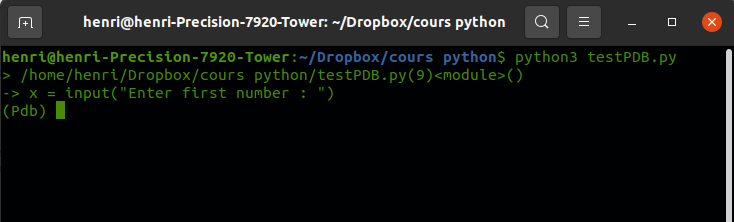
\includegraphics[width=0.5\textwidth,height=\textheight]{/home/dbhenri/Documents/Cours python/PCBS/slides/intro-to-programming/2022/8th class/screenPDB.png}
\end{frame}

\begin{frame}{Python debugger: PDB 2/4}
\protect\hypertarget{python-debugger-pdb-24}{}
\begin{itemize}
\item
  It is a command line tool that go sequentially at every step of the
  program
\item
  There are a certain number of command to know:

  \begin{itemize}
  \tightlist
  \item
    \textbf{help} To display all commands
  \item
    \textbf{where} Display the stack trace and line number of the
    current line
  \item
    \textbf{next} Execute the current line and move to the next line
    ignoring function calls
  \item
    \textbf{step} Step into functions called at the current line
  \item
    \textbf{whatis} Check the type of variable
  \end{itemize}
\end{itemize}

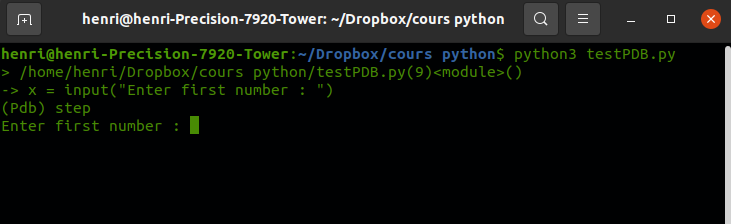
\includegraphics{/home/dbhenri/Documents/Cours python/PCBS/slides/intro-to-programming/2022/8th class/screenPDB_step.png}
\end{frame}

\begin{frame}{Python debugger: PDB 3/4}
\protect\hypertarget{python-debugger-pdb-34}{}
\begin{itemize}
\tightlist
\item
  You can use as well:

  \begin{itemize}
  \tightlist
  \item
    \textbf{args} To get all arguments of a function
  \item
    \textbf{p} To get the value at a time t of a variable
  \end{itemize}
\item
  You can navigate in pdb prompt using:

  \begin{itemize}
  \tightlist
  \item
    \textbf{c} continue execution
  \item
    \textbf{q} quit the debugger/execution
  \item
    \textbf{n} step to next line within the same function
  \item
    \textbf{s} step to next line in this function or a called function
  \item
    \textbf{u} (up)
  \item
    \textbf{d} (down)
  \end{itemize}
\end{itemize}
\end{frame}

\begin{frame}{Python debugger: PDB 4/4}
\protect\hypertarget{python-debugger-pdb-44}{}
\begin{itemize}
\item
  You can also set a breakpoint at a specific point in the script
\item
  To do that you need to write on the terminal: \textbf{break filename:
  lineno, condition}
\end{itemize}

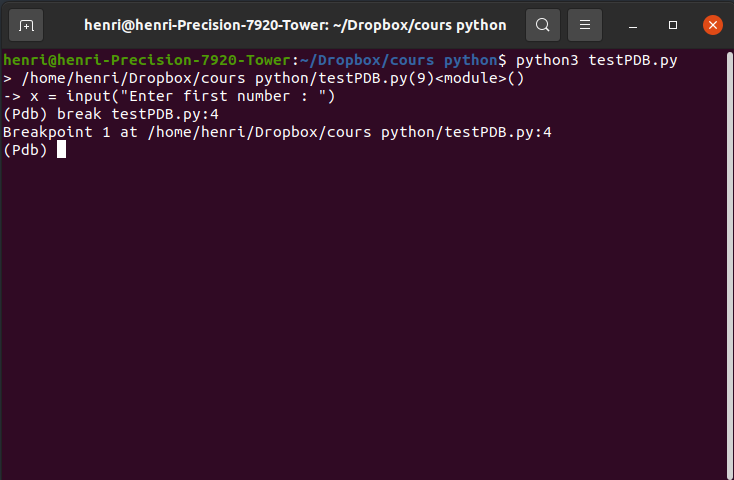
\includegraphics[width=0.5\textwidth,height=\textheight]{/home/dbhenri/Documents/Cours python/PCBS/slides/intro-to-programming/2022/8th class/screenPDB_break.png}

\begin{itemize}
\tightlist
\item
  You can then use \textbf{c} to run the program until your breakpoint
\end{itemize}

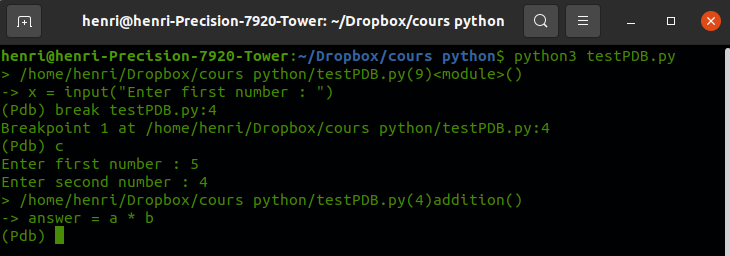
\includegraphics[width=0.5\textwidth,height=\textheight]{/home/dbhenri/Documents/Cours python/PCBS/slides/intro-to-programming/2022/8th class/screenPDB_break2.png}
\end{frame}

\end{document}
